\section{Benchmark d'unité arithmétique}\label{sec:kg}



\subsection{Introduction}
%%%%%%%%%%%%%%%%%%%%%%%%%%%%%%%%%%%%%%%%%%%%%%%%%%%%%
   
     
    La principale opportunité pour construire un supercalculateur exaflopique va être l'utilisation d'architectures hétérogènes. Ceci sera possible notamment grâce à Gen-Z. De nouveaux accélérateurs différents de ceux que nous connaissons vont être disponibles. La nécessité de les caractériser est à l'origine de ce premier outil.

    \subsubsection{Motivations}
    
    Les applications HPC exécutent, pour la grande majorité, des instructions sur des nombres réels. L'exécution de ces opérations dites \textit{flottantes} est réalisée par un composant appelé unité de calcul en virgule flottante (FPU). La performance des applications est donc dépendante de celle de ces accélérateurs. La performance de la majorité des applications est limitée par la performance du système mémoire et les efforts de développement se sont en grande partie consacrés à la caractérisation de cette partie de l’architecture. Cependant, avec ces nouvelles architectures, la différence de performance entre les unités de calculs et celle du système mémoire devrait être plus équilibrée. Il est donc important d'avoir les outils nécessaires pour les caractériser.
    Bien que le comportement des FPU des architectures actuelles soit connu,  certaines particularités sont encore difficiles à caractériser (exécution dans le désordre, dépendances entre instructions, fréquence atteignable pour un type d'instruction vectorielle). 
    Il est nécessaire de connaître la performance maximale d'un processeur (mesurée en FLOP) pour différents types de calculs. Celle-ci peut alors être utilisée pour apprécier les performances d'un code grâce à des modèles de type Roof line (voir \autoref{sec:roofline}). Pour obtenir cette performance maximale, certaines techniques utilisent les caractéristiques matérielles pour la calculer. Cependant, la complexité des architectures nous a souvent montré que la performance réellement atteignable pouvait être différente (inférieure, mais parfois aussi supérieure). En utilisant un benchmark, il est aussi possible de trouver des comportements cachés de l'architecture ou d'en déceler des limitations. 
    Le benchmark présenté utilise le langage assembleur. Ce choix a été motivé par la volonté de s'assurer que les instructions générées étaient bien exécutées. En effet, les compilateurs deviennent toujours plus performants et optimisent les codes rendant l'analyse de performance plus difficile. De plus, ils peuvent comprendre l'artificialité d'un code et contourner son exécution. En générant nous même le code assembleur, nous nous assurons que la performance du code mesuré est bien celle attendue.
    


   
    
    
    
    \subsubsection{Floating Point Unit (FPU)}
    %%%%%%%%%%%%%
        La FPU est un composant majeur des ordinateurs et a connu de nombreuses évolutions au fil des générations. À l'origine, les FPU étaient des composants additionnels pouvant être ajoutés sur la carte mère pour accélérer l'exécution de calcul en virgule flottante (\autoref{pic_cpu_fpu}\footnote{\url{https://en.wikipedia.org/wiki/Floating-point_unit}}). C'est pour cela qu'il est commun de designer ce composant comme un accélérateur. Cependant, les applications réalisant de plus en plus de calculs de ce type, les FPU ont ensuite été directement intégrées au processeur (\autoref{pic_cpu_fpu_recent}\footnote{\url{https://www.extremetech.com/computing/263963-intel-reverses-declares-skylake-x-cpus-two-avx-512-units}}). Ceci a notamment permis de réduire les latences. De plus, avec l'apparition de plates-formes multiprocesseurs, la gestion d'erreurs et d'exceptions liées aux FPU était devenue très difficile. Le premier processeur Intel à posséder une FPU et un CPU sur la même puce est le processeur Intel 80486DX produit en 1989.

        Aujourd'hui, les FPU sont des composants de haute performance permettant d'exécuter des calculs sur des nombres réels grâce à des instructions vectorielles. La FPU reçoit ses instructions du même décodeur que celui de l'unité de calcul pour les nombres entiers (ALU). Lorsque les premiers étages du pipeline (voir \autoref{sec:pipeline}) ont décodé l'instruction à exécuter, le séquenceur choisi si elle doit être exécutée l'ALU ou la FPU. 
        Les FPU sont un des composants les plus importants de l'architecture. Les applications de HPC réalisent beaucoup de calculs sur nombres flottants qui sont exécutés par les unités de calcul flottant. Ces unités sont très sollicitées et il est important d'en connaître les caractéristiques: débit, latence, fréquence maximale soutenable par le processeur. En effet, les instructions vectorielles les plus longues utilisent plus de transistors pour être utilisées. Ainsi, la chaleur émise par le processeur varie et généralement les instructions les plus longues ne peuvent être exécutées aux fréquences maximales du processeur. Les différentes fréquences atteignables pour un type d'instruction peuvent être difficiles à prévoir.
        Les modèles tels que celui du \textit{roof line} (voir \autoref{sec:roofline}), ont besoin de ces caractéristiques pour pouvoir comparer la performance mesurée d'une application à celle théoriquement atteignable. 
        

        

        \begin{figure}
            \centering
            \begin{subfigure}[b]{0.45\linewidth}
                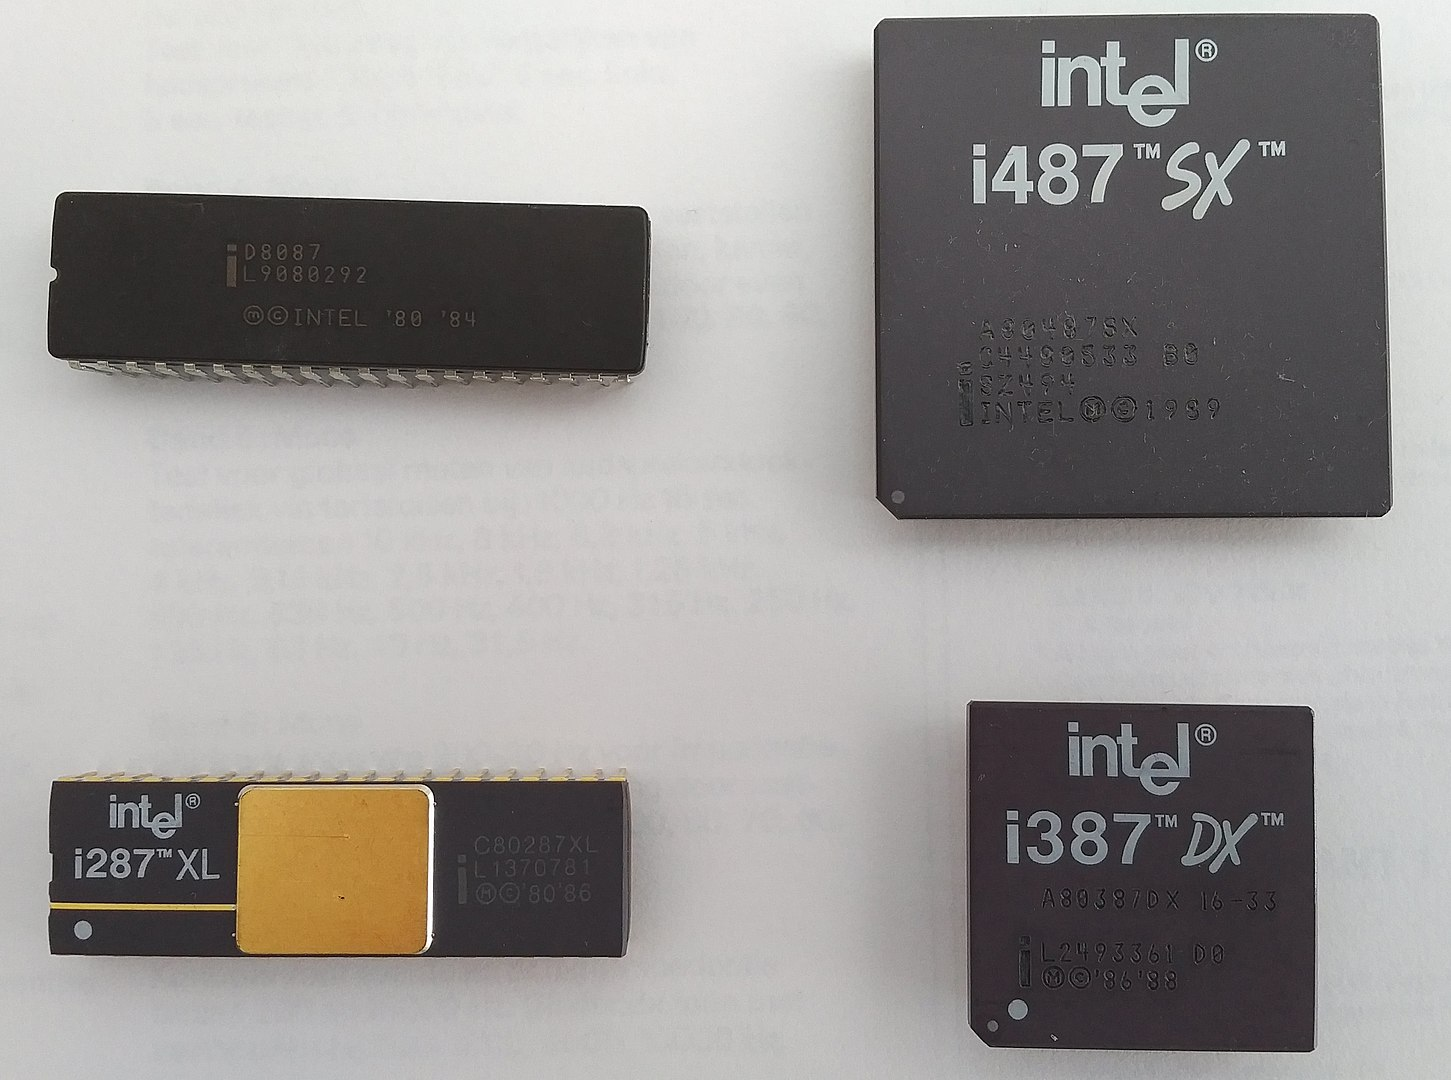
\includegraphics[width=\linewidth]{images/cpu_fpu.jpg}
                \caption{Différentes FPU qui pouvaient être achetées séparément des processeurs.}
                \label{pic_cpu_fpu}
            \end{subfigure}
            ~ %add desired spacing between images, e. g. ~, \quad, \qquad, \hfill etc. 
              %(or a blank line to force the subfigure onto a new line)
            \begin{subfigure}[b]{0.45\linewidth}
                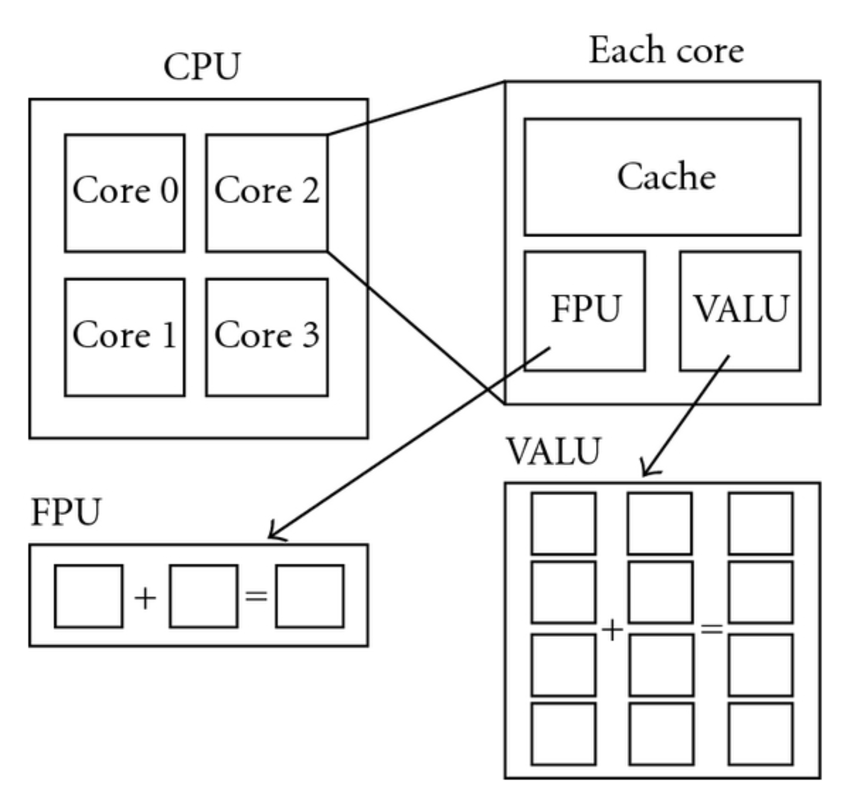
\includegraphics[width=\linewidth]{images/cpu_fpu_recent.png}
                \caption{Aujourd'hui la FPU est positionnée directement sur chaque coeur du processeur.}
                \label{pic_cpu_fpu_recent}
            \end{subfigure}
            \caption{La FPU d'un processeur est un co-processeur permettant d'exécuter efficacement des instructions de calculs arithmétiques. }\label{fig:cacheinclusionpolicy}
        \end{figure}
        
       
 
        

    
    \subsubsection{Objectifs}
    %%%%%%%%%%%%%
    
        L'objectif principal de cet outil est de caractériser finement les performances des unités de calcul en virgule flottante (FPU). 
        La première caractéristique pouvant être mesurée est la performance maximale atteignable par la FPU pour un certain type d'instruction. Cette performance est mesurée en $FLOPS$ et peut être mesurée pour des types et des tailles d'instructions différentes. L'avantage de cette unité est de rendre les résultats du Kernel Generator comparable avec ceux d'autres benchmarks (tel que \textit{HPL}). 
        La deuxième caractéristique mesurable est la latence des instructions. Il peut être intéressant de connaître celle-ci lors de l'exécution d'instructions dépendantes.
        D'autres comportements doivent être caractérisés pour anticiper la performance de certaines applications. Parmi eux, celui de l'unité d'exécution dans le désordre. Certains codes comportant beaucoup de dépendances sont limités par la faculté du processeur à exécuter plusieurs chaînes de dépendances. Cet outil vise plus particulèrement les développeurs d'application dont la performance est limitée par l'exécution d'instructions de calcul (\textit{compute bound}). Bien que la performance des processeurs soit souvent limitée par la bande passante mémoire, une partie significatives des codes est purement \textit{compute bound}. L'outil du \textit{Kernel Generator} est principalement destiné pour ce type d'applications.


        
\subsection{Kernel Generator}    
%%%%%%%%%%%%%%%%%%%%%%%%%%%%%%%%%%%%%%%%%%%%%%%%%%%%%

        Nous proposons un outil permettant de générer des kernels de calculs en assembleur pour caractériser finement le comportement des FPU. Pour expliquer son comportement, ce chapitre utilise principalement des processeurs Intel Xeon Skylake, mais le but de l'outil est d'être utilisé pour caractériser des microarchitectures différentes. 
        L'outil proposé est un générateur de benchmarks qui permet de trouver la performance crête d'un processeur pour un type d'instruction vectorielle utilisant différentes configurations (type d'instructions, dépendances...).
        
        

    \subsubsection{Concept}
    %%%%%%%%%%%%%%%%%%%%%%

            L'outil \textit{Kernel Generator} a été construit pour répondre aux objectifs fixés dans la section précédente. Il permet de tester les caractéristiques de la FPU d'un processeur grâce à l'exécution d'un kernel écrit en assembleur comportant des instructions de calcul arithmétique. Les instructions utilisées peuvent être scalaires ou vectorielles. La version actuelle de l'outil supporte les instructions de types scalaire, SSE, AVX2 et AVX512. 
            Grâce à ses différentes options, l'utilisateur peut générer des kernels d'instructions de types et de tailles différents. La valeur de l'outil vient de son utilisation et des différents tests que le programmeur peut réaliser. Le \textit{Kernel Generator} n'est pas un benchmark qu'il suffit d'exécuter pour obtenir des résultats. Cet outil respecte notre démarche initiale qui est de donner les outils à l'utilisateur pour l'aider dans son travail de profilage des applications et de caractérisation des architectures. 
            L'outil peut aussi être utilisé pour détecter des problèmes de la microarchitecture lors de l'exécution intensive d'instructions de calculs. Détecter ces comportements cachés peut ensuite permettre de mieux apprécier la performance d'une application réelle. 
        
     
        
            La \autoref{pic_kg_workflow} montre les étapes majeures de l'exécution du générateur de kernel. L'utilisateur exécute le générateur en utilisant les différentes options présentées dans la \autoref{sec:kg_option}. À partir des arguments le générateur écrit un programme en langage C++ qu'il compile et exécute. Les résultats sont ensuite présentés sous forme de texte dans le terminal ou sous forme de graphique (nécessite python). 
        
    
            \begin{figure}
            \center
            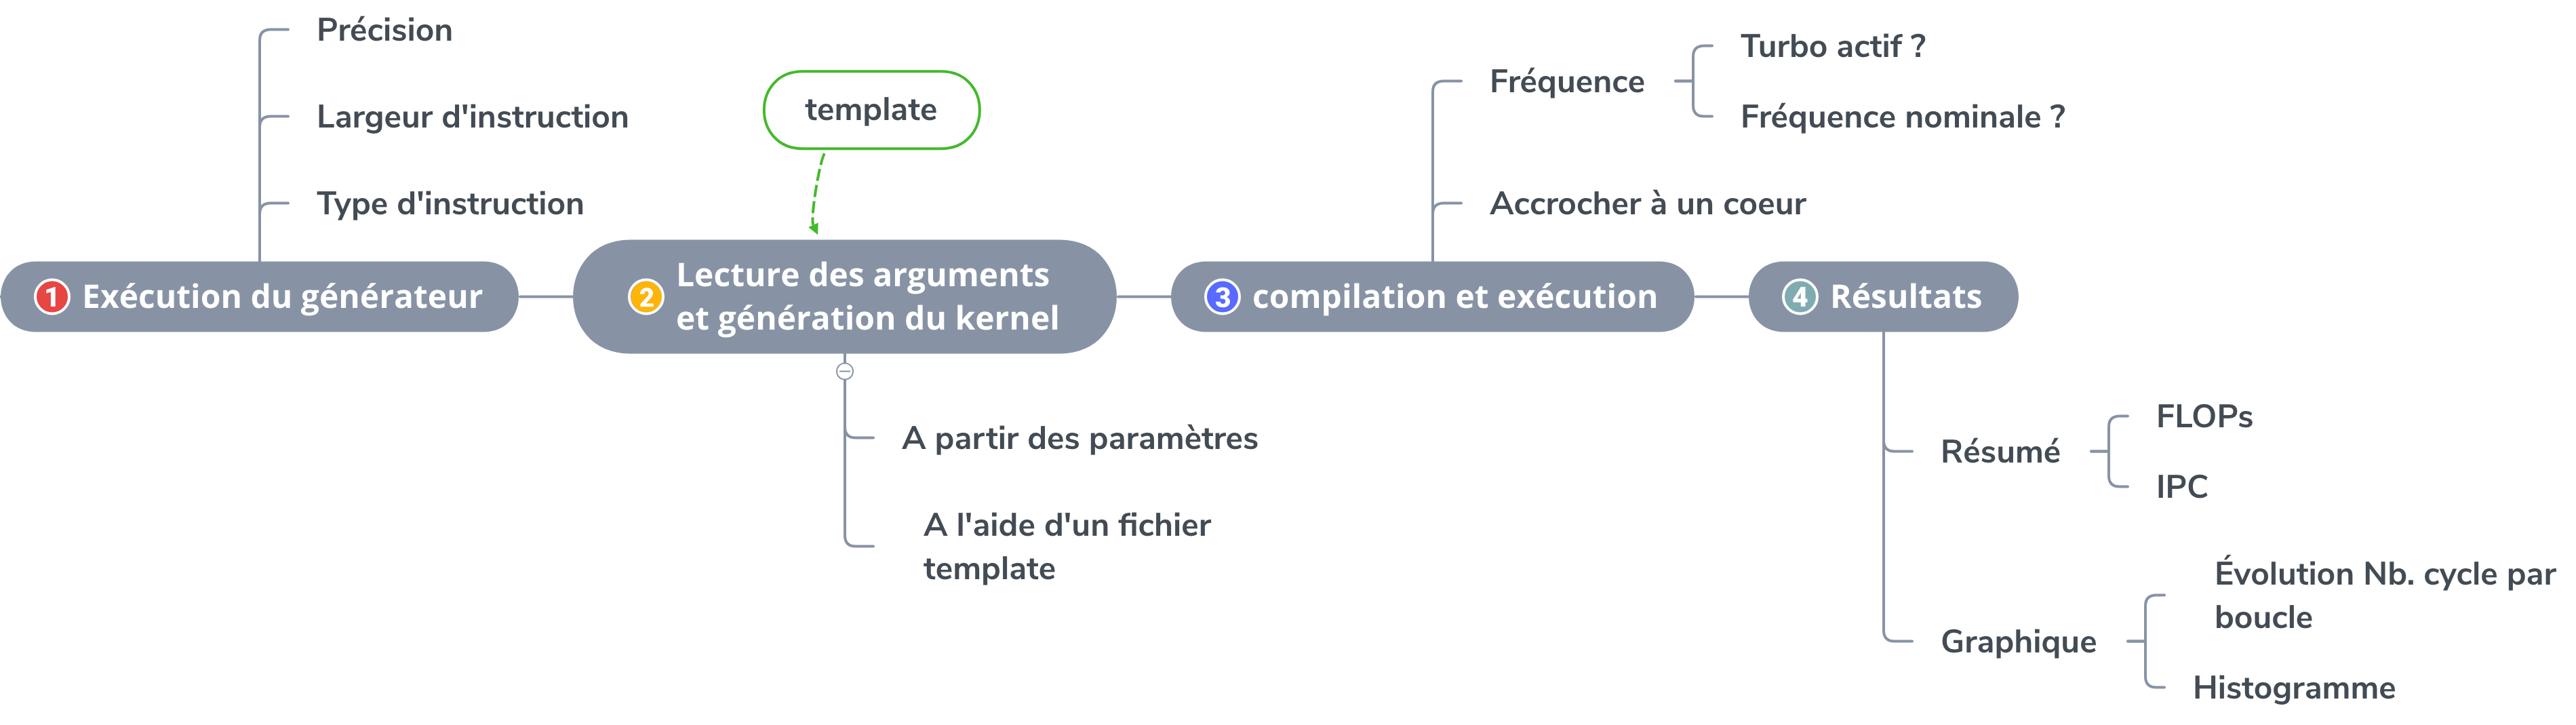
\includegraphics[width=16cm]{images/kg_workflow.png}
            \caption{\label{pic_kg_workflow} Déroulement de l'exécution du générateur de kernels.}
            \end{figure}
    
            Le générateur de kernels accepte plusieurs options lui permettant de produire différents benchmarks. La commande suivante montre un exemple d'utilisation du générateur: \verb|./kg   -P double -W 128  -O aamm|. Cette commande permet de générer un kernel de calculs utilisant quatre instructions vectorielles de 128 bits sur des nombres flottants en double précision. Le kernel est composé de quatre instructions (deux additions et deux multiplications):
        \begin{verbatim}
"vaddpd %%xmm0, %%xmm1, %%xmm2;"
"vaddpd %%xmm0, %%xmm1, %%xmm3;"
"vmulpd %%xmm0, %%xmm1, %%xmm4;"
"vmulpd %%xmm0, %%xmm1, %%xmm5;"
        \end{verbatim}
        
      
        
    
    \subsubsection{Génération du benchmark}
    %%%%%%%%%%%%%%%%%%%%%%
        
        Une fois les différentes options analysées, le générateur va écrire un programme C++ contenant le benchmark à exécuter. Tous les benchmarks ont une partie commune de code qui est stockée dans un fichier \textit{template}. Le générateur s'occupe seulement d'écrire la partie en assembleur dans ce fichier et d'initialiser quelques variables (nombre de mesures, coeur sur lequel s'exécuter). Le \textit{template} contient le code permettant de mesurer les résultats, de calculer la fréquence et d'afficher le résultat  dans le terminal. Un exemple d'exécution du générateur est résumé sur la \autoref{pic_kg_generation}. Le code généré par l'outil reste simple pour faciliter les conclusions que pourra tirer son utilisateur. En effet, produire un code trop complexe rendrait l'analyse des résultats trop difficile sur des  architectures aussi complexes que celles étudiées. 

        \begin{figure}[h!]
            \center
            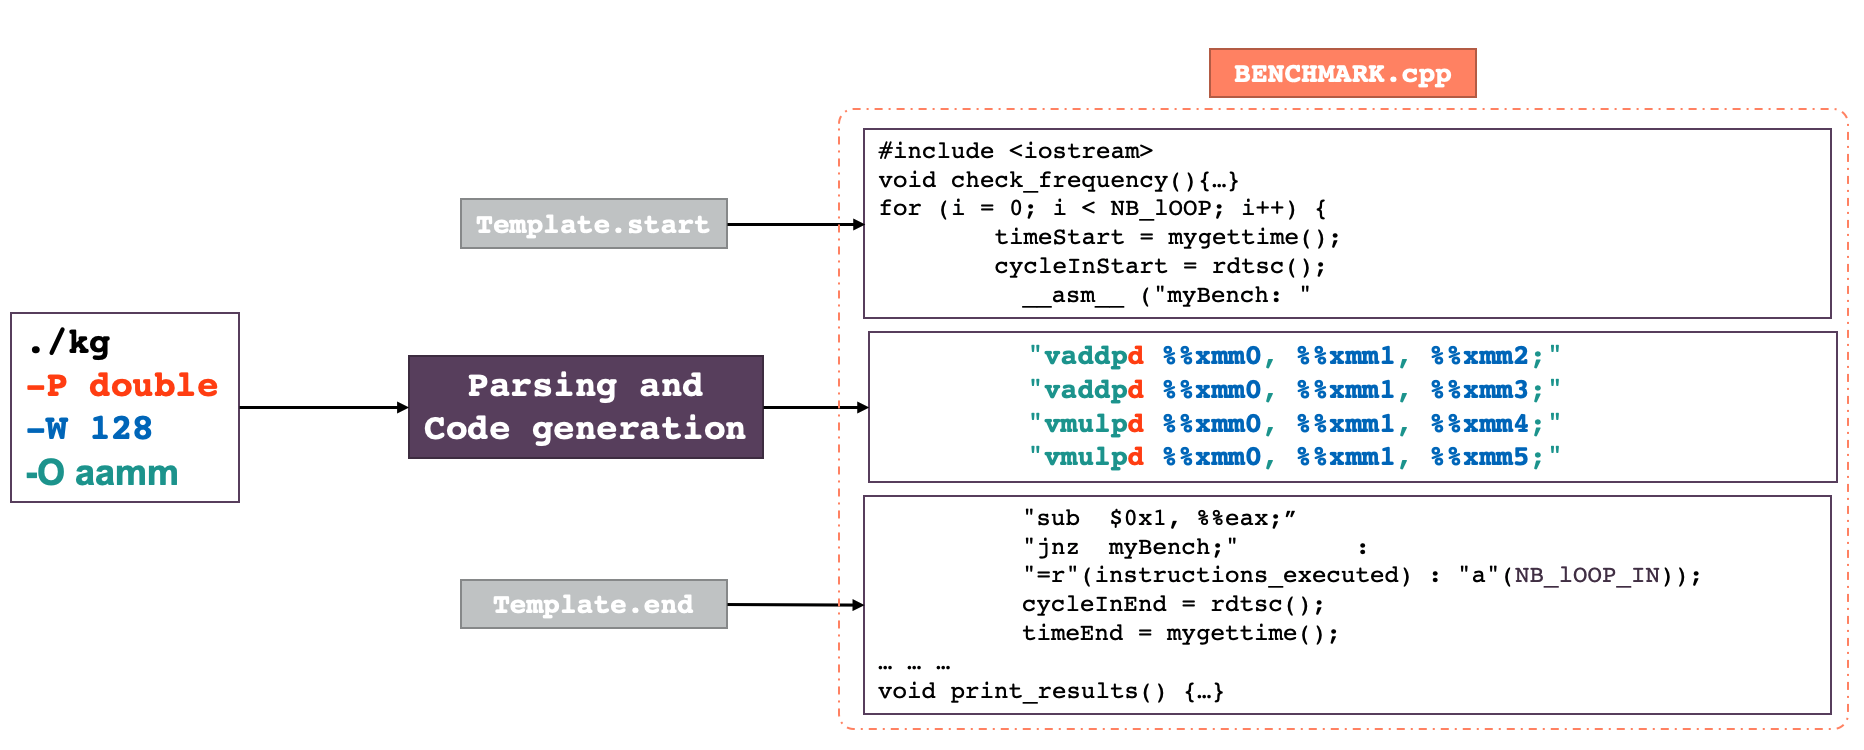
\includegraphics[width=16cm]{images/kg_generation.png}
            \caption{\label{pic_kg_generation}Génération du benchmark à partir de la ligne de commande entrée par l'utilisateur. La partie commune du code est stockée dans un fichier de \textit{template}.}
        \end{figure}
        

    \subsubsection{Exécution du benchmark}
    %%%%%%%%%%%%%%%%%%%%%%

        Une fois le code du benchmark généré (voir \autoref{pic_kg_generation}), celui-ci est compilé automatiquement par le générateur (le compilateur peut être modifié facilement). Le code et le benchmark peuvent ensuite être utilisés  sans passer de nouveau par le générateur. Ces deux fichiers sont créés dans le dossier courant de l'utilisateur. Un exemple de résultat de l'exécution du benchmark est présenté ci-dessous:
    
    
 \begin{lstlisting}[label=output:basic_gflops ,language=, caption=Exemple d'exécution d'un benchmark de quatre instructions AVX-512.]
./kg -W 512 -O aamm -P double -U 4 -S 30000 -L 500000

--------------------  CHECK FREQUENCY  ------------------------
+ Base      frequency is 2.69GHz
+ Current   frequency is 2.68GHz
+ OK: the core is running at his frequency based value

------------------  INSTRUCTIONS SUMMARY -----------------------
_label_|   NB INSTRUCTIONS      Time    FREQUENCY       Giga_inst/sec       IPC
_value_|      240000000000      44.7         2.69                5.37      1.99

----------------------  FLOP SUMMARY  --------------------------
 PRECISION     FLOP/cycle         FLOP/second
    Single              0                   0
    Double             16             4.3e+10
----------------------------------------------------------------


\end{lstlisting}   
    
        Le benchmark généré comporte quatre instructions vectorielles AVX-512: deux additions et deux multiplications. Le processeur utilisé est un  Intel Xeon 6150 cadencé à 2.70GHz. Pour cette expérimentation le turbo a été désactivé. Pour améliorer la précision des résultats, la boucle générée est déroulée 4 fois. La boucle réalise 500000 itérations et sa performance est mesurée 30000 fois. Le CPU est capable d'exécuter deux opérations flottantes vectorielles par cycle d'horloge. Pour des données en doubles précisions, cela correspond à réaliser 16 opérations flottantes par cycle. La puissance de calcul atteinte par le benchmark généré est de 43 GFLOPs. Pour chaque mesure le nombre de cycles et le temps nécessaire à l'exécution de la boucle sont sauvés dans un fichier. Ce fichier peut ensuite être affichée avec un script python (voir \autoref{fig:kg_graph}). La \autoref{pic_kg_plot} permet de voir comment la performance du benchmark évolue au fil des exécutions. On peut détecter des problèmes de détérioration des performances pouvant être dus à un mauvais refroidissement du processeur par exemple.  La \autoref{pic_kg_hist} affiche l'histogramme permettant de voir deux familles de performances.
        
        \begin{figure}
            \centering
            \begin{subfigure}[b]{0.45\linewidth}
                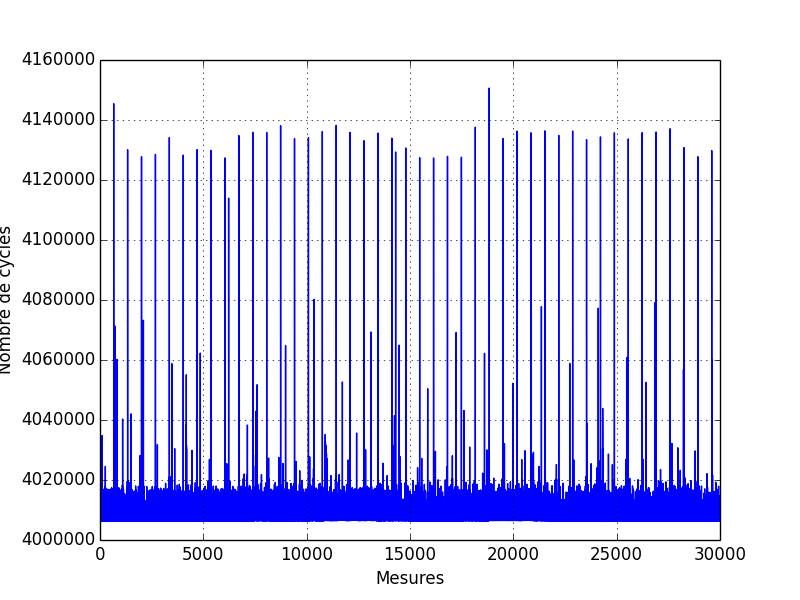
\includegraphics[width=\linewidth]{images/kg_plot.png}
                \caption{Évolution du nombre de cycles nécessaire pour l'exécution de la boucle de benchmark}
                \label{pic_kg_plot}
            \end{subfigure}
            ~ %add desired spacing between images, e. g. ~, \quad, \qquad, \hfill etc. 
              %(or a blank line to force the subfigure onto a new line)
            \begin{subfigure}[b]{0.45\linewidth}
                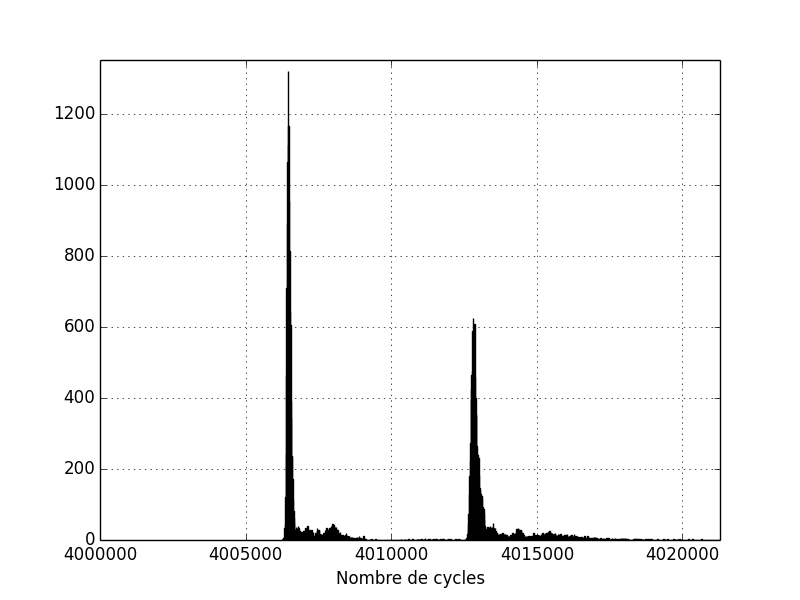
\includegraphics[width=\linewidth]{images/kg_hist.png}
                \caption{Histogramme du nombre de cycles nécessaire}
                \label{pic_kg_hist}
            \end{subfigure}
            \caption{Grâce à un script python, le fichier de résultat peut être affiché sous forme de graphique. }\label{fig:kg_graph}
        \end{figure}
    
  
        %%%% OPTION %%%    
        \subsubsection{Les options.} 
        
            Une des forces du générateur vient de sa faculté à générer un grand nombre de benchmarks différents. Ceci est possible grâce à l'utilisation des différentes options dont les principales sont expliquées dans cette sous-section.
        
            Grâce à l'option \verb|--operation {a,m,f}| l'utilisateur donne une chaîne de caractères pour choisir  les opérations à réaliser (addition (a), multiplication (m) ou FMA (f)). Différentes opérations peuvent être mixées et sont ensuite exécutées dans le même ordre. Dans cet exemple, les quatre instructions sont composées de deux additions et de deux multiplications. Cette option associée à un second script permet de générer des kernels testant différentes combinaisons d'opérations en changeant la chaîne de caractère, composée de \textit{a, m} ou \textit{f}. En faisant varier à la fois les opérations et la taille des instructions, l'outil permet de découvrir des comportements cachés des architectures.
    
            Le benchmark peut être exécuté pour réaliser des calculs en simple ou double précision grâce à l'option \verb|--precision {single, double}|. 
            La largeur des instructions vectorielles est choisie grâce à l'option \verb|--width {64, 128, 256, 512}|. Elles peuvent utiliser différentes ISA: MMX (64), SSE (128), AVX (256) ou AVX-512 (512). 
            
            L'option \verb|--dependency {N}| permet de générer une instruction  dont un opérande est le résultat produit par l'instruction précédente. Un nombre $N$ peut être donné pour générer plusieurs chaînes de dépendances non dépendantes entre elles. Cette option est particulièrement utile pour mesurer la latence des instructions et la performance du tampon d'exécution dans le désordre.
            
            L'option \verb|--binding N| est utilisée pour accrocher le benchmark généré à un coeur spécifique. Le benchmark n'étant pas parallélisé il est nécessaire d'en exécuter plusieurs versions en parallèle pour tester la performance d'un processeur lorsque plusieurs coeurs sont utilisés.
            
            L'option \verb|--unroll N| permet d'appliquer l'optimisation du déroulement de boucle N fois. Cette optimisation permet de dérouler plusieurs fois le corps de la boucle à l'intérieur de celle-ci pour réduire l'impact du traitement des instructions de contrôle de la boucle (incrémentation et comparaison) sur les performances du benchmark. 
            
            L'option \verb|--frequency| permet de générer et d'exécuter une fonction en début de benchmark qui mesure la fréquence du processeur. Les calculs des résultats sont impactés par l'utilisation du mode turbo. En connaissant la valeur de la fréquence turbo, ces résultats peuvent être ajustés. En effet, la mesure de la performance du benchmark est réalisée en utilisant la valeur de la fréquence de base du processeur. 
            
            Pour améliorer la précision des résultats et éliminer les potentiels bruits de mesure, l'utilisateur peut indiquer le nombre $N$ de mesures à réaliser grâce à l'option \verb|--loopsize N|.    
    
    
    \subsubsection{Validation des résultats}
    
        Lors du développement du générateur, il a été nécessaire d'utiliser des outils nous permettant de valider les performances rapportées par le benchmark. Pour s'assurer du bon fonctionnement du benchmark sur de nouvelles architectures, certaines de ces méthodes de vérification ont été implémentées dans l'outil directement. 
        
        
        %#TODO enelver le compteur je pense qu'il est NDA pour HPE
        \paragraph{Validation du nombre d'instructions.} La première valeur à valider est de s'assurer que le bon nombre d'instructions a été exécuté par le benchmark. Le benchmark affiche le nombre d'instructions qui devrait être exécutées. Un moyen de le vérifier est d'utiliser les compteurs matériels. L'outil \textit{perf} permet de mesurer le nombre d'évènements d'un compteur en utilisant son adresse (une instruction FMA compte pour deux). La ligne de commande suivante permet de compter les opérations flottantes réalisées par le benchmark: \verb|perf stat -e /rffc7 ./benchmark|. Le résultat du benchmark ci-dessus prévoyait l'exécution de 240,000,000,000 opérations. La commande \verb|perf stat| retourne une valeur de 240,000,210,024 opérations. Pour comprendre d'où proviennent les instructions supplémentaires, nous avons mesuré différentes versions du benchmark avec différentes longueurs de boucle (5000, 10000 et 20000). Le \autoref{tab:kg_vs_perf} donne les résultats affichés par le benchmark et par la commande précédente utilisant l'outil \textit{perf}. Les résultats de \textit{perf} mesure le bon nombre d'instructions avec 2124 opérations supplémentaires à chaque fois. Ces instructions supplémentaires correspondent en fait au traitement des résultats..
    
        \begin{table}[h!]
        \centering
        \resizebox{\textwidth}{!}{%
        \begin{tabular}{@{}lcc@{}}
        \toprule
         & Nombre d'instructions & Résultat perf \\ \midrule
        ./kg -W 512 -O aamm -P double -S 300 -L 5000 & 6000000 & 6002124 \\
        ./kg -W 512 -O aamm -P double -S 300 -L 10000 & 12000000 & 12002124 \\
        ./kg -W 512 -O aamm -P double -S 300 -L 20000 & 24000000 & 24002124 \\ \bottomrule
        \end{tabular}%
        }
        \caption{Vérification du nombre d'instructions exécutées avec l'outil perf.}
        \label{tab:kg_vs_perf}
        \end{table}
        
        
        
        \paragraph{Validation de l'IPC.} La validation de l'IPC peut elle aussi être réalisée grâce à perf et la commande \verb|perf stat ./benchmark|. Pour générer le benchmark la commande suivante a été utilisée: \verb|./kg -W 512 -O aamm -P double -S 1000 -L 90000000|. Pour que les instructions vectorielles prennent la plus grande partie du temps de l'exécution, la taille de la boucle a été allongée. Le benchmark donne alors un IPC de 2 alors que la commande \textit{perf} donne un résultat de 3. Cette différence peut être expliquée en regardant le code assembleur généré (voir \autoref{lst:kg:ipc}). 
        
        \begin{lstlisting}[label=lst:kg:ipc ,language=C, caption=Code généré par la commande ./kg -W 512 -O aamm -P double]
cycleInStart = rdtsc();
__asm__ ("" 
    "myBench: " 
		"vaddpd %%zmm0, %%zmm1, %%zmm2; "
		"vaddpd %%zmm0, %%zmm1, %%zmm3; "
		"vmulpd %%zmm0, %%zmm1, %%zmm4; "
		"vmulpd %%zmm0, %%zmm1, %%zmm5; "
    "sub  $0x1, %%eax;"
    "jnz  myBench;"		: "=r" (instructions_executed) : "a" (NB_lOOP_IN));
cycleInEnd = rdtsc();
\end{lstlisting}
        
        Notre calcul d'IPC ne prend en considération que les instructions de calculs alors que \textit{perf} compte la totalité des instructions exécutées. Notre calcul prend pour postulat que les deux instructions de gestion de boucle (la décrémentation \verb|sub|, et le saut conditionnel \verb|jnz|) ne rentre pas dans le profil de l'exécution. Grâce au prédicateur de branchement, l'instruction de saut peut effectivement être enlevée de nos calculs. Concernant la soustraction, nous avons réalisé un test pour vérifier l'impact de soustraction de nombre entier lors de l'exécution d'un code ne réalisant que des opérations sur des nombres flottants (voir \autoref{code:sub}). 
        
        \begin{lstlisting}[label=code:sub ,language=C, caption=Mesure de l'impact de la soustraction]
"myBench: " 
 "vfmadd231pd %%zmm0, %%zmm1, %%zmm2; "
 "vfmadd231pd %%zmm0, %%zmm1, %%zmm3; "
 "vfmadd231pd %%zmm0, %%zmm1, %%zmm4; "
 "vfmadd231pd %%zmm0, %%zmm1, %%zmm5; "
 "sub  $0x1, %%ebx;" //fake substraction
 "sub  $0x1, %%ebx;" //fake substraction
 "sub  $0x1, %%ebx;" //fake substraction
 "sub  $0x1, %%eax;" 
"jnz  myBench;"	  
        \end{lstlisting}
        
        
        En mesurant la performance de ce code, nous avons mesuré que 4 soustractions sur des nombres entiers n'impactent pas la performance de la boucle. Au-delà de 4, le processeur a besoin de cycles supplémentaires pour les exécuter. Ainsi les deux instructions de gestion de boucles peuvent être ignorées de notre calcul. Pour réduire l'impacte de ces deux instructions sur le résultat donnée par \textit{perf}, nous avons implémenté une option de déroulement de boucle (\textit{unrolling}). La commande suivante déroule le code 10 fois permettant de valider le calcul d'IPC du benchmark avec la valeur donnée par \textit{perf}: \verb|kg -W 512 -O aamm -P double -S 10 -L 900000000 -U 10 |.
        
        
        
        
        \paragraph{Validation des FLOPS.} La première méthode a été d'utiliser un outil développé en interne appelé \textit{mygflops}. Cet outil affiche le nombre d'opérations exécutées en consultant les compteurs matériels de chaque coeur. Le résultat sépare les différentes tailles d'instructions vectorielles utilisées. La commande, le résultat du benchmark et celui de \textit{mygflops} sont présentés dans l'\autoref{lst:basic_gflops}. 
        
\begin{lstlisting}[label=lst:basic_gflops ,language=C, caption=Validation des résultats donnés par le benchmark grâce à l'outil \textit{mygflops}.]
./kg -W 128 -O aamm -P double -U 10 -S 10 -L 90000000
...
----------------------  FLOP SUMMARY  --------------------------
 PRECISION     FLOP/cycle         FLOP/second
    Single              0                   0
    Double           4.00            1.06e+10
----------------------------------------------------------------
...

********************** MYGFLOPS ***********************
     
Single-precision SSE/AVX :            0.000000 GFlop/s --  0.0% of Flops

       0.0%  32-bit SSE/AVX instructions (0.0%)
       0.0% 128-bit SSE/AVX instructions (0.0%)
       0.0% 256-bit AVX instructions     (0.0%)
       0.0% 512-bit AVX instructions     (0.0%)
     
Double-precision SSE/AVX :            10.572521 GFlop/s -- 100.0% of Flops

       0.0%  64-bit SSE/AVX instructions (  0.0%)
     100.0% 128-bit SSE/AVX instructions (100.0%)
       0.0% 256-bit AVX instructions     (  0.0%)
       0.0% 512-bit AVX instructions     (  0.0%)

\end{lstlisting}
        
        Cependant, cet outil n'est pas disponible en accès libre pour le reste de la communauté. Nous avons ainsi développé une méthode de validation des résultats interne au benchmark. En fonction des opérations utilisées, les registres sont initialisés avec différentes valeurs significatives. Par exemple, pour vérifier que le bon nombre d'additions a été exécuté, les registres sont initialisés à la valeur 1. À la fin du benchmark, les registres ayant participé au benchmark sont sommés pour vérifier que le bon nombre d'additions a été exécuté. Grâce à cette méthode, nous avons la certitude que les opérations sont réellement exécutées par le processeur et qu'aucune optimisation lui permettant d'en éviter n'est possible ou une erreur de logique.
        

    
    \subsubsection{Mesure de la fréquence}
    %%%%%%%%%%%%%%%%%%%%%%
        Plus un processeur utilise une fréquence élevée, plus sa consommation électrique est élevée. Pour cette raison, Intel a adopté différents niveaux de fréquences pour ses processeurs. Cela permet d'augmenter les performances en cas de besoin et de limiter la consommation d'énergie si le processeur n'a pas besoin d'être pleinement utilisé. L'instruction \verb|rdtsc| est utilisée pour lire le compteur matériel correspondant au nombre de \textit{tics} depuis la dernière réinitialisation du processeur \cite{code:rdtsc}. La fréquence correspond à la fréquence de base nominale du processeur est indépendante de la fréquence d'horloge réelle pouvant varier. Si les fréquences des processeurs devaient varier, les mesures effectuées avec \verb|rdtsc| seraient erronées. C'est pourquoi la fréquence du processeur doit être choisie avant l'exécution du micro-benchmark. Dans le cas d'une fréquence fixe différente de la fréquence de base nominale, nous avons mis en place une vérification qui calculera ensuite cette fréquence, et ajustera les résultats mesurés par \verb|rdtsc| comme le calcul de l'IPC. Cette fonctionnalité de vérification de la fréquence et de la correction de résultat est utilisable avec l'option \verb|-F true|. 
        
        \paragraph{Mesurer la fréquence de base.} Nous avons développé un code pour mesurer la fréquence de base. Il utilise la fonction \textit{sleep} qui attend un certain nombre de microsecondes ainsi que l'instruction \verb|rdtsc|. Ainsi nous pouvons calculer la fréquence avec le rapport $cycleSpent / timeSpent$ comme indiqué sur \autoref{code:base_freq}. 
        

\begin{lstlisting}[label=code:base_freq ,language=C, caption=Code used to measure the base frequency of the processor]
timeStart = mygettime();
cycleInStart = rdtsc();
    usleep(10000);
cycleInEnd = rdtsc();
timeEnd = mygettime();
cycleSpent = (cycleInEnd - cycleInStart);
freq_Base = cycleSpent / (1000000000 * (timeEnd - timeStart));
\end{lstlisting}        

        \paragraph{Mesurer la fréquence réelle.} Pour pouvoir ajuster les résultats affichés par le benchmark, il est nécessaire de connaître la fréquence à laquelle le processeur est capable d'aller. Cette fréquence peut varier en fonction de l'utilisation du mode \textit{turbo} ou si la fréquence a été limitée de façon logicielle. Pour réaliser cette mesure, nous sommes partis du constat que tous les processeurs modernes sont capables d'exécuter une soustraction sur un registre par cycle d'horloge. Dans l'\autoref{code:cur_freq}, le registre \verb|%eax| est initialisé à \verb|80000000|. Grâce à notre hypothèse, il est possible de prévoir que le processeur réalisera ces \verb|80000000| soustractions en autant de cycles. Nous mesurons le nombre de cycles à \textit{fréquence nominale} passé dans l'exécution de cette boucle. En faisant le rapport entre le nombre de cycles mesurés et celui attendu grâce à notre hypothèse, il est possible de déterminer si le processeur utilise une fréquence plus ou moins rapide que sa fréquence nominale. Nous calculons ainsi l'IPC de cette boucle en faisant le rapport $\frac{80000000}{cycleSpent}$.
        \begin{itemize}
            \item \verb|IPC == 1|: Le processeur utilise sa fréquence de base
            \item \verb|IPC < 1|: Le processeur utilise une fréquence inférieur à sa fréquence de base.
            \item \verb|IPC > 1|: Le processeur est capable d'exécuter des instructions à une fréquence plus élevée que sa fréquence de base (turbo).
        \end{itemize}
    
\begin{lstlisting}[label=code:cur_freq ,language=C, caption=Mesure de la fréquence de base du processeur]
cycleInStart = rdtsc();
__asm__ ("aloop: "
    "sub $0x1,%%eax;"
    "sub $0x1,%%eax;"
    "sub $0x1,%%eax;"
    "sub $0x1,%%eax;"
    "jnz aloop" : : "a" (80000000UL)
);
cycleInEnd = rdtsc();
cycleSpent = (cycleInEnd - cycleInStart);
\end{lstlisting}   
    
    
        \paragraph{Ajuster les résultats.} En connaissant la fréquence de base et la fréquence accessible par le processeur les résultats donnés par le benchmark peuvent être ajustés. Nous avons utilisé un script externe pour verrouiller la fréquence du processeur Intel Xeon 6150 à 2.00 GHz. Ce processeur a une fréquence de base de 2.70GHz. Notre code présenté dans la section précédente mesure un IPC pour le code du \autoref{code:cur_freq} de 0.742. Cela signifie qu'il fonctionne actuellement à 74,2\% de sa fréquence de base, soit 2,00 GHz. Ce premier test permet de valider la méthodologie basée sur \verb|rdtsc|, mais aussi pour valider avant toute expérimentation que la fréquence est correctement réglée. Grâce à l'option \verb|--frequency true| le générateur fera cette vérification pour ajuster les résultats donnés par \verb|rdtsc|. 
        
    
    
    
    
    
    
\subsection{Résultats}
%%%%%%%%%%%%%%%%%%%%%%%%%%%%%%%%%%%%%%%%%%%%%%%%%%%%%
    Nous présentons dans cette section comment le générateur peut être utilisé pour caractériser une plate-forme ainsi que les résultats obtenus pendant les travaux de thèse.
   
   
   

    \subsubsection{Vérifier les performances théoriques}
    %%%%%%%%%%%%%%%%%%%%%%%%%%%%%%%%%%%%%%%%%%%%%%%%%%%%%
    Le générateur de kernels peut être utilisé pour vérifier ou mesurer les performances maximales atteignables par un processeur. Pour illustrer cette utilisation, nous avons étudié les performances du processeur Intel Xeon 6150 cadencé à 2.7 GHz, possédant 18 coeurs et disposant d'un mode Turbo. Les résultats de cette expérimentation sont donnés dans le \autoref{tab:kg_vs_intel}. Pour chaque configuration (nombre de coeurs, type d'instructions, turbo activé) Intel donne dans sa documentation les différentes fréquences supportées par le processeur\footnote{\url{https://www.intel.com/content/dam/www/public/us/en/documents/specification-updates/xeon-scalable-spec-update.pdf}}. Lorsque le turbo est désactivé, la fréquence du processeur pour exécuter un type d'instructions ne varie pas en fonction du nombre de coeurs utilisés. Cette fréquence est appelée \textit{Base Core Frequency} (BCF). Cette fréquence est également la fréquence minimale qui peut être atteinte par un processeur doté d'un système de refroidissement correctement configuré. Cette fréquence peut donc être utilisée pour calculer une limite inférieure de la performance du processeur. Cependant la fréquence BCF donnée par Intel est une fréquence garantie. Si la température et la conception du processeur le permettent, le processeur peut utiliser des fréquences plus élevées. Le but de cette expérimentation est d'utiliser le générateur de kernel pour mesurer cette fréquence et ainsi déterminer la performance maximale théorique lorsque le turbo est désactivé. 
    Pour connaître la borne supérieure de la performance maximale du processeur, il faut lire attentivement la documentation pour en relever les valeurs présentées sur la quatrième ligne du \autoref{tab:kg_vs_intel} (colonne \textit{Turbo ON}). Cette fréquence est appelée \textit{Maximum Core Frequency} (MCF). Cette fréquence n'est pas garantie, et est seulement atteignable si la température du processeur le permet. En fonction de sa qualité de fabrication (fuite de courant) et de l'efficacité de son système de refroidissement, la fréquence MCF peut varier de 20\%.  

    
    La performance maximale atteignable (en GFLOPs) pour chaque type d'instructions (Non-AVX, AVX 2.0 et AVX-512) peut être mesurée en exécutant des instructions FMA. Nous avons utilisé le générateur de kernel pour créer des benchmarks utilisant trois tailles d'instructions (scalaire, 256 et 512 bits) avec la commande suivante:
\begin{lstlisting}
./kg -W {64,256, 512} -O ffffffffffffff -P double -U 80 -S 1 -L 90000000
\end{lstlisting}


    \begin{table}[h!]
    \centering
    \resizebox{\textwidth}{!}{%
    \begin{tabular}{|l|cc|cc|cc|cc|cc|cc|}
    \hline
    Jeu d'instruction & \multicolumn{4}{c|}{\cellcolor[HTML]{67FD9A}Non-AVX} & \multicolumn{4}{c|}{\cellcolor[HTML]{34FF34}AVX 2.0} & \multicolumn{4}{c|}{\cellcolor[HTML]{009901}AVX 512} \\ \hline
    Turbo & \multicolumn{2}{c|}{\cellcolor[HTML]{FFFFC7}OFF} & \multicolumn{2}{c|}{\cellcolor[HTML]{FCFF2F}ON} & \multicolumn{2}{c|}{\cellcolor[HTML]{FFFFC7}OFF} & \multicolumn{2}{c|}{\cellcolor[HTML]{FCFF2F}ON} & \multicolumn{2}{c|}{\cellcolor[HTML]{FFFFC7}OFF} & \multicolumn{2}{c|}{\cellcolor[HTML]{FCFF2F}ON} \\ \hline
    Nombre de coeurs & \multicolumn{1}{c|}{\cellcolor[HTML]{ECF4FF}1} & \cellcolor[HTML]{CBCEFB}18 & \multicolumn{1}{c|}{\cellcolor[HTML]{ECF4FF}1} & \cellcolor[HTML]{CBCEFB}18 & \multicolumn{1}{c|}{\cellcolor[HTML]{ECF4FF}1} & \cellcolor[HTML]{CBCEFB}18 & \multicolumn{1}{c|}{\cellcolor[HTML]{ECF4FF}1} & \cellcolor[HTML]{CBCEFB}18 & \multicolumn{1}{c|}{\cellcolor[HTML]{ECF4FF}1} & \cellcolor[HTML]{CBCEFB}18 & \multicolumn{1}{c|}{\cellcolor[HTML]{ECF4FF}1} & \cellcolor[HTML]{CBCEFB}18 \\ \hline
    \rowcolor[HTML]{EFEFEF} 
    Fréquence (GHz) (source Intel) & 2.7 & 2.7 & 3.7 & 3.4 & 2.3 & 2.3 & 3.6 & 3.0 & 1.9 & 1.9 & 3.5 & 2.5 \\ \cline{1-1}
    \rowcolor[HTML]{EFEFEF} 
    Performance théorique (GFLOPs) & 10.8 & 194.4 & 14.8 & 244.8 & 36.8 & 662.4 & 57.6 & 864 & 60.8 & 1094 & 112 & 1440 \\ \hline
    \rowcolor[HTML]{FFE4E2} 
    Performance KG (GFLOPs) & 10.8 & 192.6 & 14.8 & 244.2 & 43 & 772.2 & 57.3 & 858.8 & 86 & 1430 & 112 & 1430 \\ \cline{1-1} 
    \rowcolor[HTML]{FFE4E2} 
    Fréquence calculée (GHz) & 2.7 & 2.7 & 3.7 & 3.4 & {\color[HTML]{00009B} \textbf{2.68}} & {\color[HTML]{00009B} \textbf{2.68}} & 3.58 & {\color[HTML]{000000} 2.97} & {\color[HTML]{00009B} \textbf{2.68}} & {\color[HTML]{00009B} \textbf{2.48}} & 3.5 & 2.48 \\ \hline
    \end{tabular}%
    }
            \caption{
            Mesure de la performance du processeur Intel 6150 utilisant trois jeux d'instructions, avec et sans Turbo et en utilisant un seul ou tous les coeurs. Les données mesurées (en rouge) sont à comparer avec les spécifications techniques données par le constructeur (en gris). Intel communique les fréquences minimales garanties pour chaque cas. Cependant, les performances réelles peuvent être supérieures (en bleu) lorsque le processeur est capable de soutenir une fréquence plus élevée (consommation électrique, chaleur).}
            \label{tab:kg_vs_intel}
    \end{table}
    
    
    Quelle que soit la taille de l'instruction, le processeur Skylake étudié est capable d'exécuter deux instructions par cycle. Ces instructions nécessitant plus ou moins de transistors pour être exécutées (taille, nombre de coeur) le processeur doit adapter sa fréquence pour ne pas surchauffer.  Le Kernel Generator mesure le nombre d'instructions par cycle, ce qui nous permet de vérifier que deux instructions FMA sont bien exécutées chaque cycle. Le benchmark calcule aussi la performance en GFLOPs du code. Grâce à ces deux informations, il est possible de calculer la fréquence réelle qu'utilise le processeur (dernière ligne du  \autoref{tab:kg_vs_intel}). Nous remarquons en bleu, quatre fréquences supérieures à celles annoncées par la documentation. En effet, Intel communique la fréquence minimale garantie pour chaque configuration (turbo, nombre de coeurs, type d'instructions). Cette fréquence minimale est garantie pour tous les processeurs d'un même modèle (même SKU). La qualité de fabrication du processeur peut lui permettre d'atteindre des fréquences plus élevées que celle-ci, comme indiqué en bleu dans le \autoref{tab:kg_vs_intel}. Pour étudier l'évolution de la fréquence et de la température du processeur, nous utilisons un outil développé en interne par HPE. La \autoref{pic_kg_freq_vs_temp} montre que le processeur est capable d'utiliser une fréquence de 2.7 GHz, alors que la fréquence minimale garantie est de 2.3 GHz. Le benchmark a été exécuté pendant trente minutes. Le bon système de refroidissement utilisé empêche le processeur de dépasser sa puissance TDP (Thermal Design Power) et conserve cette fréquence durant toute l'exécution. La puissance TDP est mesurée en watt et exprime la quantité de chaleur dégagée par le processeur lorsqu'il est en charge. Le TDP permet au constructeur de systèmes de refroidissement de calibrer le matériel nécessaire pour refroidir un processeur.  
    
           
    \begin{figure}[!h]
        \centering
        \begin{subfigure}[t]{0.45\linewidth}
            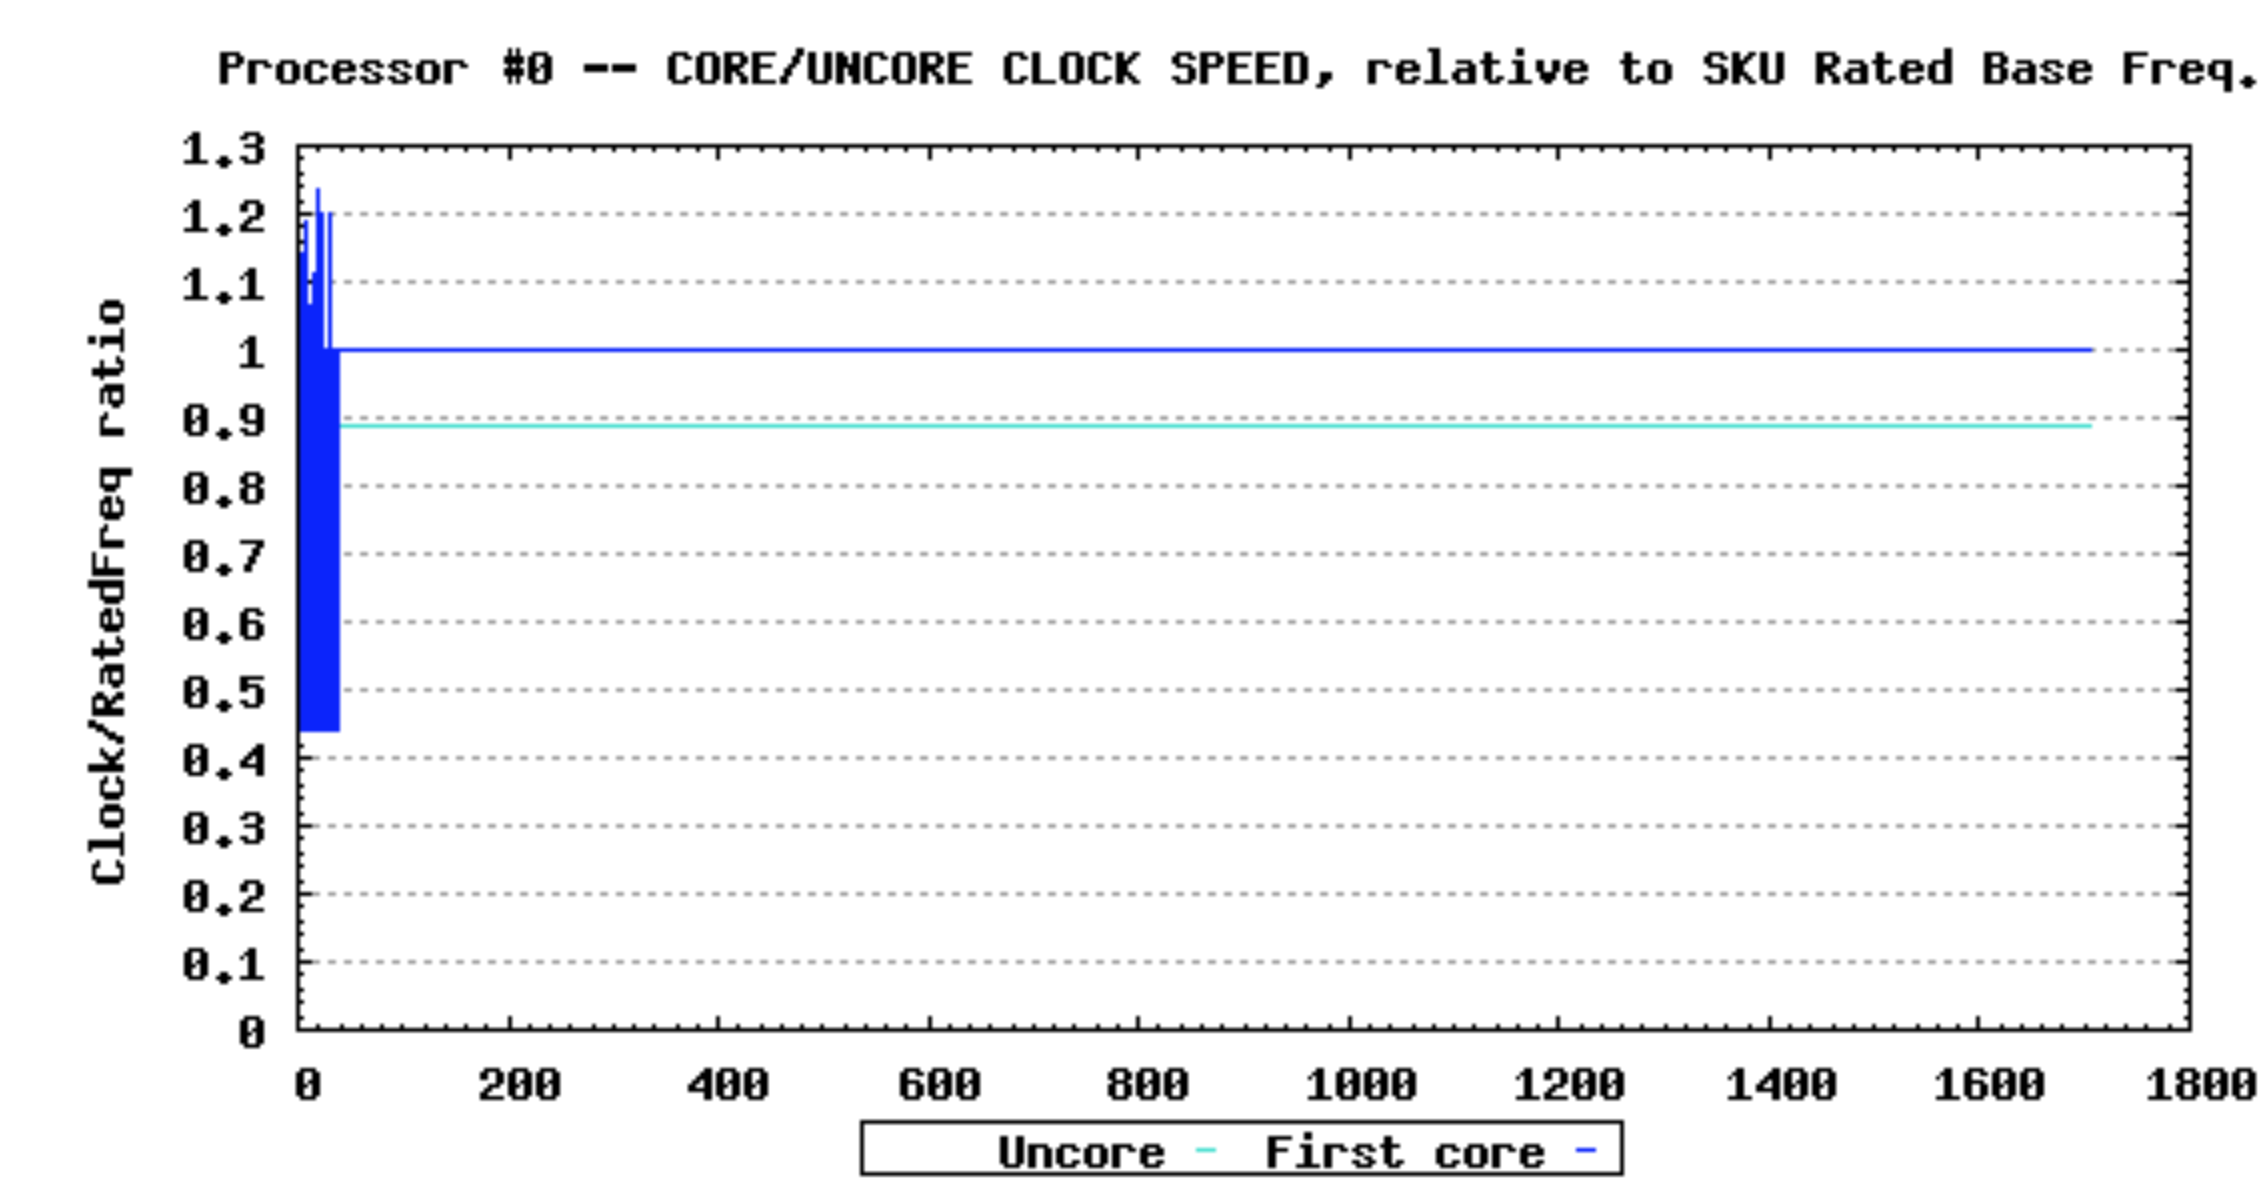
\includegraphics[width=\linewidth]{images/kg_freq.png}
            \caption{Évolution de la fréquence. Un ratio de 1 correspond à la fréquence de base de processeur (2.7 GHz).}
            \label{pic_kg_freq}
        \end{subfigure}
        ~ %add desired spacing between images, e. g. ~, \quad, \qquad, \hfill etc. 
          %(or a blank line to force the subfigure onto a new line)
        \begin{subfigure}[t]{0.45\linewidth}
            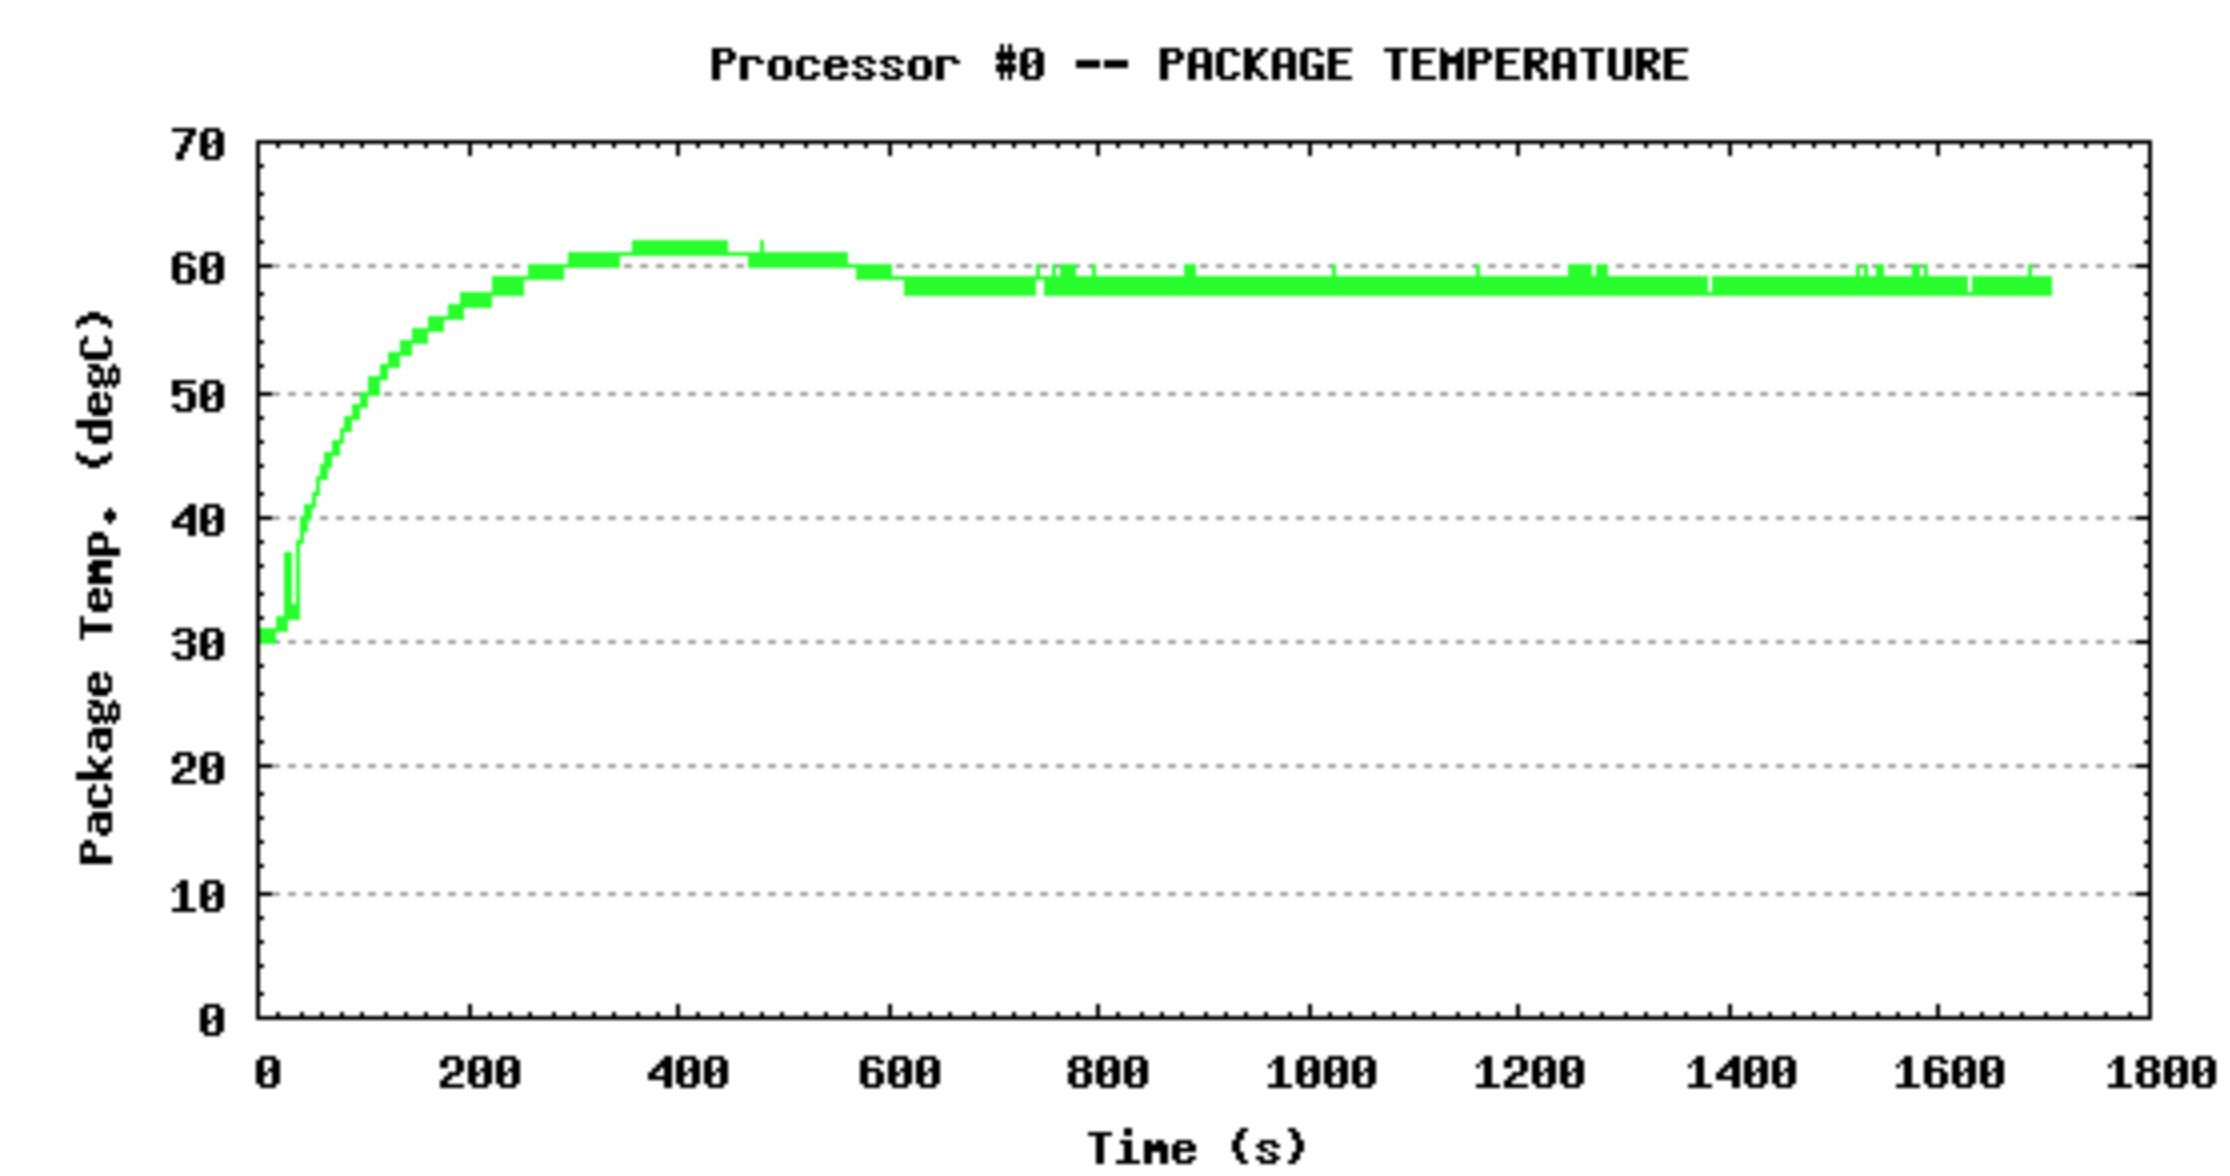
\includegraphics[width=\linewidth]{images/kg_temp.png}
            \caption{Évolution de la température du processeur}
            \label{pic_kg_temp}
        \end{subfigure}
        \caption{Évolution de la fréquence et de la température du processeur pour un benchmark AVX 2.0 exécuté sur 18 coeurs avec le turbo désactivé}\label{pic_kg_freq_vs_temp}
    \end{figure}

        




    
    \subsubsection{Caractérisation de la micro-architecture Haswell}
    %%%%%%%%%%%%%%%%%%%%%%%%%%%%%%%%%%%%%%%%%%%%%%%%%%%%%
    Lors de l'utilisation d'une nouvelle plate-forme, l'utilisateur peut utiliser le générateur de benchmarks pour caractériser la microarchitecture et trouver ses points forts ou points faibles. Lors de l'arrivée des processeurs Intel de génération Haswell en 2013, certains codes ont connu des baisses de performances malgré l'utilisation d'une architecture plus récente. Nous avons utilisé le générateur de kernels pour caractériser les performances d'exécution des additions et des multiplications avec la commande suivante : \verb|./kg  -P double -W 64 -O mmmmm| permettant de générer le benchmark suivant:
    
    \begin{lstlisting}[label=lst:kg_mul ,language=C]
for (i = 0; i < NB_lOOP; i++) {
timeStart = mygettime();
cycleInStart = rdtsc();
__asm__ ("" 
     "myBench:"  
   		"vmulsd %%xmm0, %%xmm1, %%xmm2; "
   		"vmulsd %%xmm0, %%xmm1, %%xmm3; "
   		"vmulsd %%xmm0, %%xmm1, %%xmm4; "
   		"vmulsd %%xmm0, %%xmm1, %%xmm5; "
   		"vmulsd %%xmm0, %%xmm1, %%xmm6; "
     "sub  $0x1, %%eax;"
     "jnz  myBench;"		:: "a" (NB_lOOP_IN));
cycleInEnd = rdtsc();
timeEnd = mygettime();
cycle_total += (cycleInEnd - cycleInStart);
time_total += timeEnd - timeStart;
}
\end{lstlisting}
    
     La microarchitecture Haswell est capable d'exécuter deux multiplication par cycle. Cependant, l'utilisation du générateur de kernel nous a montré que le processeur n'était pas capable d'exécuter des additions au même rythme que les multiplications. Les résultats présentés dans le \autoref{tab:mul_vs_add} montrent que la microarchitecture Haswell est capable d'exécuter deux multiplications contre une seule addition par cycle.

    \begin{table}[h!]
    \centering
    \begin{tabular}{|l|c|c|c|c|}
        \hline
        Opération & Nombre d'instructions & Frequence & Temps & IPC \\ \hline
        Multiplication & 40000000000 & 2.1 & 7.71 & \textbf{2} \\ \hline
        Addition & 40000000000 & 2.1 & 14.43 & {\color[HTML]{963400} \textbf{1}} \\ \hline
        \end{tabular}%
        
        \caption{Différence de performance lors de l'exécution d'addition et de multiplication sur une architecture Haswell.}
        \label{tab:mul_vs_add}
    \end{table}
    
    Bien sûr, cette caractéristique est documentée et en comptant le nombre de ports destinés aux additions, l'utilisateur du processeur aurait pu en trouver la raison. Cependant la lecture de la documentation de la microarchitecture dépasse le millier de pages et en comprendre les moindres détails est plus difficile que d'utiliser les bons outils. Nous pensons que le générateur de benchmarks peut permettre à n'importe quel utilisateur de rapidement trouver ce genre de caractéristiques. Avant même d'avoir exécuté son application sur une nouvelle plate-forme, il peut rapidement se faire une idée de ses performances et trouver ce genre de défauts.




    \subsubsection{Caractérisation de l'exécution dans le désordre}
    %%%%%%%%%%%%%%%%%%%%%%%%%%%%%%%%%%%%%%%%%%%%%%%%%%%%%

    La puissance d'un supercalculateur vient de sa capacité à réaliser des calculs en parallèle. Pour satisfaire la loi d'Amdahl (voir \autoref{sec:amdhal}), les développeurs essaient de maximiser les zones de codes pouvant profiter des ressources parallèles des architectures. Le principal frein à l'utilisation du parallélisme vient de zones de codes dit séquentiels. Ces lignes de codes doivent être exécutées à la suite les unes des autres, car par exemple, une de ces instructions nécessite d'avoir le résultat de la précédente. Les performances d'un tel code peuvent être très mauvaises, mais la nature des algorithmes peut assez fréquemment laisser place à certaines optimisations. Dans le domaine des finances, les algorithmes de Monte-Carlo sont très utilisés. Ces codes ont la particularité d'exposer de longues chaînes de dépendances. En restructurant le code, le programmeur peut espérer profiter de l'exécution dans le désordre (voir \autoref{sec:out_of_order}). Cela nécessite cependant d'apporter suffisamment d'instructions indépendantes au processeur pour qu'il puisse les exécuter en parallèle. Le processeur est capable d'exécuter plusieurs chaînes indépendantes les unes des autres. La performance d'une telle plate-forme dépend alors de sa capacité à en exécuter plusieurs en parallèle. Grâce à l'option \verb|--dependency N| du générateur de kernels, le benchmark peut être utilisé pour caractériser cette fonctionnalité matérielle. Cette option permet de générer plusieurs chaînes indépendantes. En utilisant une dépendance de 1, chaque instruction a besoin du résultat de l'instruction précédente (voir \autoref{lst_dep1}). Dans ce cas-là, aucune parallélisation n'est possible pour le processeur.
    
    
\begin{lstlisting}[label=lst_dep1,language=C, caption=Code généré par la commande /kg -W 512 -P double -O mmmmm -D 1]
"myBench: " 
	"vmulpd %%zmm0, %%zmm6, %%zmm2; "
	"vmulpd %%zmm0, %%zmm2, %%zmm3; "
	"vmulpd %%zmm0, %%zmm3, %%zmm4; "
	"vmulpd %%zmm0, %%zmm4, %%zmm5; "
	"vmulpd %%zmm0, %%zmm5, %%zmm6; "
"sub  $0x1, %%eax;"
"jnz  myBench;"
\end{lstlisting}

    La performance atteinte par ce code est de 0.25 instruction par cycle d'horloge. Le processeur a besoin de 4 cycles d'horloge pour exécuter une instruction. Cette latence vient de la nécessité d'attendre que le résultat de l'opération précédente soit disponible pour pouvoir commencer à être exécutée. 
    
    En ajoutant des chaînes de dépendances grâce à l'option \verb|--dependecy N|, nous avons pu valider que le processeur est capable d'exécuter au moins 8 chaînes d'instructions indépendantes. Le code généré pour 4 chaînes est présenté sur la \autoref{pic_kg_dep_4}. En faisant varier le nombre de chaînes indépendantes, les résultats présentés dans le \autoref{tab_kg_depth} ont été obtenus. Grâce au tampon d'instructions de système d'exécution dans le désordre, le processeur est capable de commencer l'exécution de plusieurs chaînes indépendantes simultanément. Le processeur peut exécuter une multiplication par cycle par pipeline (2 au total). La latence d'une multiplication AVX-512 étant de 4 cycles, le processeur a besoin de 8 chaînes indépendantes pour utiliser la totalité de la puissance du processeur. Cette caractéristique du processeur doit être connue par le programmeur pour transformer son code et obtenir le maximum de performance du processeur. Grâce au générateur de kernels, les nouvelles architectures peuvent être testées pour caractériser ces performances et prévoir leur performance pour des codes pouvant utiliser des chaînes de calculs indépendantes comme la résolution de polynômes par exemple. 
    
         \begin{figure}
            \center
            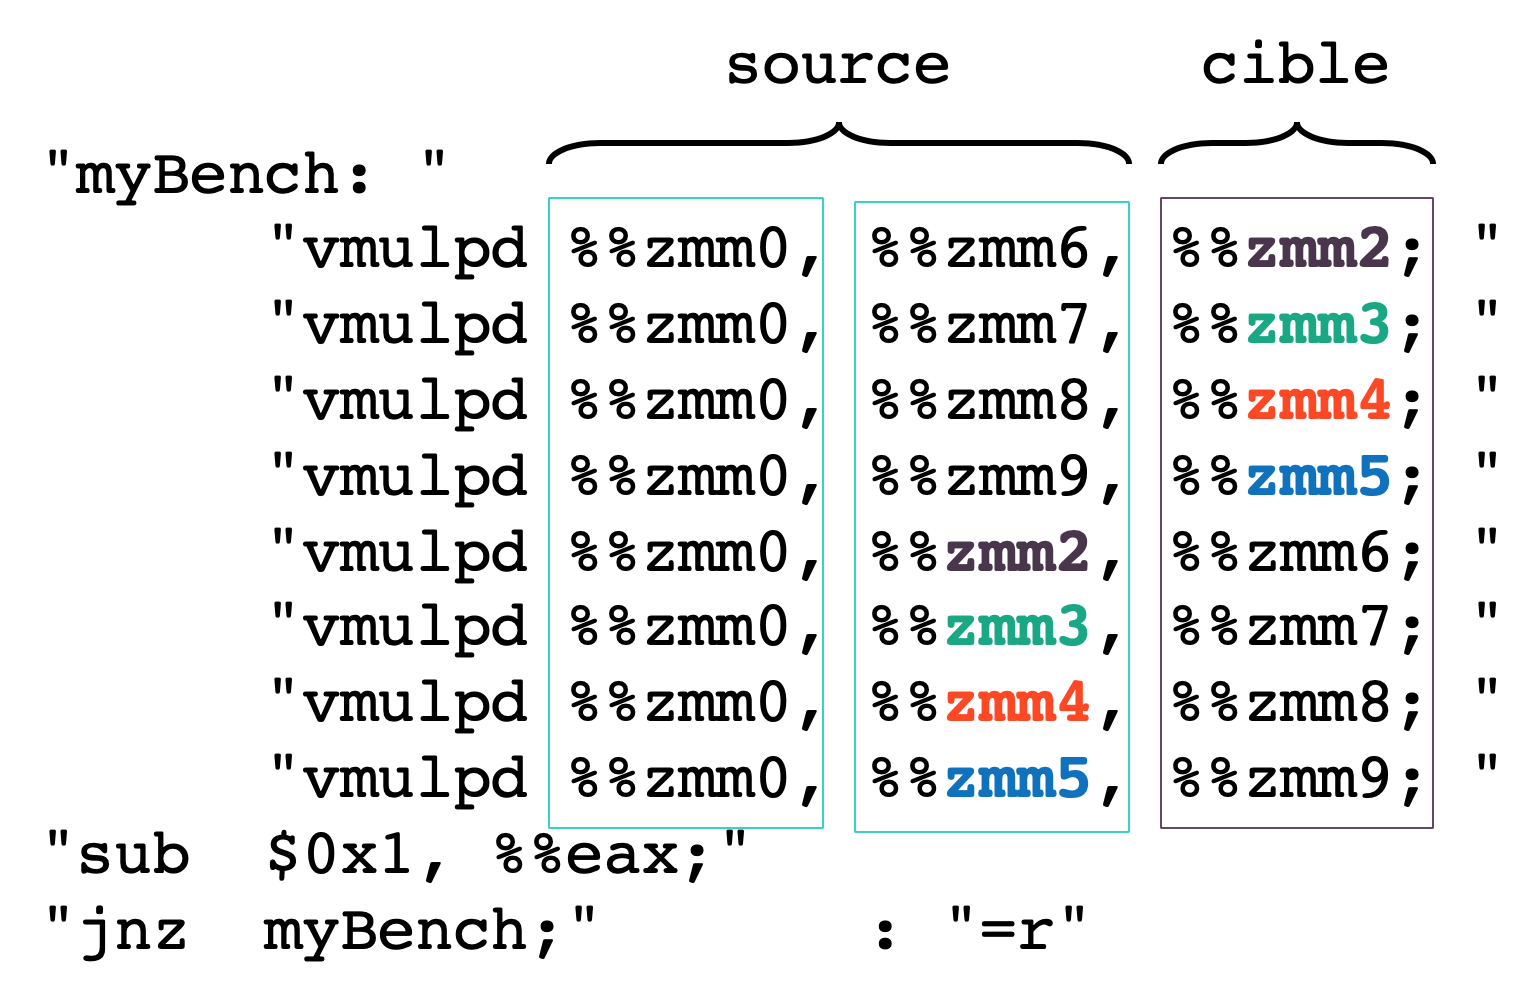
\includegraphics[width=8cm]{images/kg_dep_4.png}
            \caption{\label{pic_kg_dep_4} Code généré par la commande /kg -W 512 -P double -O mmmmmmmm -D 4}
        \end{figure}

    \begin{table}[h!]
    \centering
    \normalsize
    \begin{tabular}{|l|c|c|c|c|c|c|c|c|c|c|}
    \hline
    Nombre de chaînes & 1 & 2 & 3 & 4 & 5 & 6 & 7 & 8 & 9 & 10 \\ \hline
    IPC & 0.25 & 0.50 & 0.75 & 1 & 1.25 & 1.50 & 1.75 & 2 & 2 & 2 \\ \hline
    \end{tabular}%
    \caption{Impact du nombre de chaînes pouvant être exécutées indépendamment sur la performance du code (mesurée en Instruction Par Cycle).}
    \label{tab_kg_depth}
    \end{table}





    \subsubsection{Caractérisation de la FPU de deux processeurs Skylake}

        Pour caractériser la performance crêtes des processeurs, notre équipe de benchmark utilise des codes tels que HPL. Pour obtenir la meilleure performance atteignable, le benchmark est compilé pour utiliser les instructions vectorielles les plus grandes (AVX-512) (voir \autoref{table:skl_bench}). La dernière génération de processeur Intel Skylake est répartie en quatre gammes (bronze, silver, gold et platinium). Les fonctionnalités et les performances des processeurs des différentes gammes étant différentes (voir \autoref{table:skl}), il est important pour notre équipe avant-vente d'en connaître les caractéristiques et les performances pour adapter les configurations des serveurs aux demandes clients. Les processeurs des gammes bronze ou silver sont rarement choisis pour répondre à un appel d'offres compte tenu de leurs caractéristiques plus faibles (une FPU au lieu de deux, nombre plus faible de coeurs).
        
        
        \begin{table}[h!]
        \centering
        \caption{Skylake portfolio: différences principales des SKUs}
        \label{table:skl}
        \resizebox{\textwidth}{!}{%
        \begin{tabular}{|l|l|l|l|l|l|}
        \hline
        \rowcolor[HTML]{EFEFEF}
                                        &   Bronze: 31XX                    & Silver: 41XX              & Gold: 5100            & Gold: 6100            & Platinium: 8100           \\ \hline
        Memory channel and speed    & 6-ch@2133 Ghz                         & 6-ch\textbf{@2400}      & 6-ch@2400           & 6-ch\textbf{@2666}   & 6-ch@2666                \\ \hline
        UPI links (Scalability)         &     2   (2S-2UPI)       & 2  (2S-2UPI)    & 2 (4S-2UPI)  & 3  (2S-3UPI) & 3    (8S-3UPI)    \\ \hline
        UPI bandwidth                   & 9.6 GT/s                          & 9.6 GT/s                  & 10.4 GT/s              & 10.4 GT/s             & 10.4 GT/s                 \\ \hline
        HyperThreading  \cite{Marr2002}                &   NO                              & \textbf{YES}              & YES                   & YES                   & YES                       \\ \hline
        FMA-512 FPU                     &     1                             & 1                         & 1                     & \textbf{2 }           & 2                         \\ \hline
        
        \end{tabular}
        }
        
        \end{table}
        
        
      Les résultats du benchmark Linpack donnés dans le \autoref{table:skl_bench}, montrent que les processeurs les plus performants sont ceux appartenant aux gammes Gold et Platinium. Ces processeurs possèdent généralement plus de coeurs, et sont capables d'utiliser des fréquences plus élevées que les processeurs d'entrée de gamme. Bien sûr, comme ces processeurs coûtent plus cher à l'achat, un client choisira un processeur en fonction de son budget, de sa consommation électrique ou du profile de son application. Cette différence de performance peut être expliquée par la présence de deux FPU sur les processeurs haut de gamme. Ces deux FPU sont capables d'exécuter chacune une instruction FMA en AVX-512 par cycle. Grâce au générateur de kernel, cette caractéristique a pu être vérifiée (voir \autoref{table:skl_bench}).

        \begin{table}[h!]
        \centering
        \caption{Skylake performance the HPL Benchmark in GFLOP/s: 8 process per core, HyperThreading off, frequency capped at 1.5 Ghz) \textbf{todo: refaire full core no capping}}
        \label{table:skl_bench}
        \resizebox{\textwidth}{!}{%
        \begin{tabular}{|l|l|l|l|l|}
        \hline
        \rowcolor[HTML]{EFEFEF}
        Processeur (Nb. FPU)    & Silver: 4110 (1)  & Gold: 5117 (1)   & Gold: 6130 (2)    & Platinium: 8160 (2)        \\ \hline
        HPL (512)            & 297           & 372          & 714           & 716                  \\ \hline
        AVX-512 FMA par cycle   & 1             & 1            & 2             & 2                    \\ \hline
        \end{tabular}
        }
        \end{table}
        
        
        Afin d'estimer l'impact d'une FPU manquante sur la performance, nous avons utilisé une application de CFD typique. L'application utilisée n'exécute que des instructions vectorielles de 256 bits. Nous nous attendons alors à obtenir des performances différentes entre un processeur Silver et Gold pour une application qui n'est pas limitée par la bande passante mémoire. Étonnamment, les résultats obtenus sur ces deux plates-formes sont très proches. Pourtant, nous avons bien montré que les processeurs de gamme supérieure possèdent une FPU de plus et sont donc deux fois plus performants. 

        Pour comprendre ce phénomène, nous avons utilisé le générateur de benchmark pour générer un kernel de calculs utilisant des instructions AVX de 256 bits.    


        \begin{verbatim}
./kg  -P double -W 256 -O ffffffff -F true
        \end{verbatim}
        
        \begin{table}[h!]
        \centering
        % increase table row spacing, adjust to taste
        %\renewcommand{\arraystretch}{1.1}
        % COMMENTS if using array.sty, it might be a good idea to tweak the value of
        %\extrarowheight{1} as needed to properly center the text within the cells
        \caption{Xeon Gold and Silver results for AVX2 instructions}
        \label{table:skl_bench2}
        \resizebox{0.4\textwidth}{!}{%
        \begin{tabular}{|l|l|l|l|l|}
        \hline
        \rowcolor[HTML]{EFEFEF}
                                & Silver: 4110       & Gold: 6130      \\ \hline
        IPC                     & 2                  & 2           \\ \hline
        GFLOP/s                 & 2.38e+10           & 2.37e+10           \\ \hline
        \end{tabular}
        }
        \end{table}
        
        La performance mesurée pour le kernel AVX-2 sont reportés dans le \autoref{table:skl_bench2}.  Bien que le processeur Intel Xeon Silver 4110 ne possède qu'une seule FPU, il est capable d'exécuter deux instructions AVX-2 par cycle. Cette caractéristique peut être retrouvée dans la documentation du processeur \footnote{source: \url{https://en.wikichip.org/wiki/intel/microarchitectures/skylake\#Execution_engine_2}}. Les FPU des processeurs Skylake d'entrée de gamme fusionnent deux ports de 256 bits pour former la FPU 512-bits. Cependant, lorsque des instructions de 256 bits sont exécutées, le processeur peut utiliser les deux ports indépendamment pour exécuter deux instructions. La FPU supplémentaire sur les processeurs haut de gamme est une FPU 512 bits qui ne permet pas d'utiliser cette caractéristique et d'exécuter (en théorie) quatre instructions par cycle. 

        Nous avons ensuite poussé la caractérisation des FPU des processeur Silver plus loin pour vérifier comment la fusion de la FPU fonctionnait. Pour cela, le générateur de benchmarks a de nouveau été utilisé grâce à l'option permettant de mixer différentes tailles d'instructions vectorielles. Les résultats reportés dans le \autoref{res:skl} ont pu être trouvés. La FPU est capable chaque cycle d'exécuter: 


        \begin{itemize}
            \item Une instruction AVX 512 bits.
            \item Deux instruction AVX 256 bits.
            \item Deux instructions AVX 128 bits.
            \item Deux instructions scalaire.
            \item Toutes combinaisons de deux instructions dont la taille agrégée ne dépasse pas 512 bits.
        \end{itemize}
        
        
        \begin{table}[h!]
        \normalsize
        % increase table row spacing, adjust to taste
        %\renewcommand{\arraystretch}{1.1}
        % COMMENTS if using array.sty, it might be a good idea to tweak the value of
        %\extrarowheight{1} as needed to properly center the text within the cells
        \caption{Nombre d'instructions exécutées chaque cycle pour différentes gammes de processeurs en mixant différentes tailles d'instructions.}
        \label{res:skl}
        \centering
        %\resizebox{\textwidth}{!}{%
        \begin{tabular}{|l|c|c|c|c|}
            \hline
            \rowcolor[HTML]{EFEFEF} 
            Gamme & Silver & Gold & Gold & Platinium \\ \hline
            \rowcolor[HTML]{EFEFEF} 
            Ref. processeur Intel Skylake & 4110 & 5117 & 6130 & 8160 \\ \hline
            \rowcolor[HTML]{EFEFEF} 
            Nombre de FPU & 1 & 1 & 2 & 2 \\ \hline
            128 + scalaire & \textbf{2} & \textbf{2} & 2 & 2 \\ \hline
            256 + scalaire & \textbf{2} & \textbf{2} & 2 & 2 \\ \hline
            256 + 128 & \textbf{2} & \textbf{2} & 2 & 2 \\ \hline
            256 & \textbf{2} & \textbf{2} & 2 & 2 \\ \hline
            512 + scalaire & 1 & 1 & 2 & 2 \\ \hline
            512 + 128 & 1 & 1 & 2 & 2 \\ \hline
            512 + 256 & 1 & 1 & 2 & 2 \\ \hline
        
        \end{tabular}
        %}
        \end{table}
        
        
        
       Ainsi, le processeur haut de gamme bénéficie des deux FPU lorsque le code est capable d'utiliser des instructions vectorielles de 512 bits. Il est fréquent que les applications n'y parviennent pas (mauvaise vectorisation du code, problème du compilateur, dépendances) et utilisent des instructions vectorielles plus petites, les processeurs d'entrée de gamme obtiennent des performances rigoureusement égales. Évidement, la FPU n'est pas la seule responsable de la performance d'une application, le \autoref{table:skl} montrent bien que d'autres caractéristiques diffèrent telles que le nombre de liens UPI ou la possibilité d'utiliser l'hyperthrading . Le but du générateur de kernels est de caractériser une architecture pour le besoin d'une application. Plusieurs réponses à des offres d'appels ont été réalisées avec des processeurs d'entrée de gamme. Grâce à cette caractéristique, les applications utilisant des instructions AVX-2 peuvent obtenir des performances assez proches sur des processeurs coûtant beaucoup moins cher.


        
        




%    \subsubsection{Expliquer les performances d'un code}
    %%%%%%%%%%%%%%%%%%%%%%%%%%%%%%%%%%%%%%%%%%%%%%%%%%%%%
 %   Une autre utilisation du générateur de kernel peut permettre d'expliquer les performances d'une autre application. 
    
    
  %   What we have seen in the past months with the releases of the new Skylake processors is that entry level processors like Intel 4110 can perform as good as a top bin processor like the Intel 6148 for real applications thus increasing the $\frac{performance}{price}$ of a large scale cluster. 



    
    %%%%%%%%%%%%%%%%%%%%%%%%%%%%%%%%%%%%%%%%%%%%%%%%%%%%%



\subsection{Conclusion}
%%%%%%%%%%%%%%%%%%%%%%%%%%%%%%%%%%%%%%%%%%%%%%%%%%%%%
    
    Le générateur de kernel assembleur est un outil très précis pour la caractérisation des FPUs. Le principal avantage de l'utilisation de l'assembleur est d'éliminer les optimisations du compilateur. Le benchmark doit assurer à l'utilisateur qu'il mesure bien la performance du code qu'il a choisi de générer et qu'il n'a pas été modifié durant la compilation. Il nous a permis d'atteindre des performances souvent égales aux performances théoriques. 
    
    Pour le moment, seul l'ISA x86 est supporté, mais l'outil a été codé de façon à faciliter l'ajout d'une nouvelle ISA. Nous avons choisi de commencer à le développer pour des processeurs dont nous connaissons bien le comportement pour valider son bon fonctionnement. L'exemple de la FPU du processeur Intel Xeon 4110, nous a permis de montrer que même sur des architectures que nous connaissons bien, certaines spécificités nous échappent encore. L'utilisation du générateur permet d'en comprendre toutes les particularités.
    
    Il est connu que la performance des applications actuelles est principalement limitée par le système mémoire. Ainsi, nous avons constaté le manque d'outils permettant de caractériser les unités de calculs arithmétiques. 
    
    En utilisant le générateur, le programmeur peut être amené à découvrir des particularités de la microarchitecture (comme celle de l'exécution dans le désordre). En comprenant précisément le fonctionnement de la FPU, il pourra même trouver des optimisations pour sa propre application.
    
    La suite du travail comprend la fin du développement de l'option permettant de mixer différentes tailles d'instructions vectorielles dans le même kernel. Nous pensons aussi permettre de générer des instructions générant des déplacements mémoires pour vérifier qu'elles ne gênent pas l'exécution des instructions de calculs. Enfin, pour mieux caractériser les plate-formes pour certaines applications comme en cryptographie, nous allons ajouter d'autres instructions pouvant être générées (rotation, décalage...).